%! TEX program = xelatex
\documentclass[10pt]{article}


%\usepackage{geometry}
\usepackage[a4paper, margin=0.2in]{geometry}
\usepackage{booktabs}
\usepackage{mathrsfs}
\usepackage{epsfig}
\usepackage{helvet}
\usepackage{courier}
\usepackage{amsmath, amssymb, amsthm, amsfonts, graphicx}
\usepackage{url,color}
\usepackage{tabularx}
\usepackage{amssymb}
\usepackage{amsmath}
\usepackage{amsthm}
\usepackage{nicefrac}
\usepackage{graphicx}
\graphicspath{ {./} }
\usepackage{epsfig}


\usepackage{mdframed}
\usepackage{tabu}
\usepackage{algorithm}
\usepackage[noend]{algpseudocode}
\usepackage{wrapfig}
\usepackage{empheq}
\usepackage{ragged2e}
%\usepackage{multicol}
\usepackage{mathtools}
\usepackage{pstricks-add, auto-pst-pdf}
\usepackage{tikz}
\usepackage{textcomp}
\usetikzlibrary{positioning,chains,fit,shapes,calc}

\frenchspacing
%\newtheorem{theorem}{Theorem}
\newtheorem{note}{Note}
\newtheorem{lemma}{Lemma}
\newtheorem{prop}{Proposition}
\newtheorem{theorem}{Theorem}
\newtheorem{definition}{Definition}

\usepackage{tikz}
\usetikzlibrary{calc}
\usepackage{caption}
\setlength{\topmargin}{ 0.1in}
\setlength{\columnsep}{2.0pc}
\setlength{\headheight}{0.0in} \setlength{\headsep}{0.0in}
\setlength{\oddsidemargin}{.15in} \setlength{\parindent}{1pc}
\setlength{\evensidemargin}{.15in} \setlength{\parindent}{1pc}
\setlength{\parsep}{15pt}
\textheight 9.0in \textwidth 6.0in
\newcommand{\hr}{\noindent\rule{\textwidth}{.35mm}\vspace{8pt}}% 




\begin{document}
\begin{mdframed}

    Statistical Methods in AI 
    \hfill% move it to the right
    04.11.2019


    \begin{center}
    \begin{LARGE}
        SMAI Assignment 2 Report
    \end{LARGE}
    \end{center}
    Zubair Abid
    \hfill
    20171076
\end{mdframed}	
$ $\\

\section{Basic Questions}
\begin{enumerate}
    \item \textbf{What are eigen faces?}\\
    Eigenfaces is the name given to a set of eigenvectors when they are used in the computer vision problem of human face recognition. It is essentially an eigendecomposition of faces to lower dimensions, using multiple methods such as basic PCA, LDA, Fisherface, etc.
    
    \item \textbf{How many eigenvectors/faces are required to “satisfactorily” reconstruct a  person  in  these  three  datasets?}\\
    We do not need too many features to reconstruct a person, per se. However, to be absolutely certain, it would be correct to claim that a representation that has about 95\% of the features of the original image should be satisfactory to reconstruct a person in this three databases.\\ 
$ $\\
Going with this logic, we attempt to calculate the number of features needed by a basic PCA eigenface representation to get this approximate 95\%. IMFDB: 110 features; Yale face database: 70 features; IIIT CFW: 300 features

    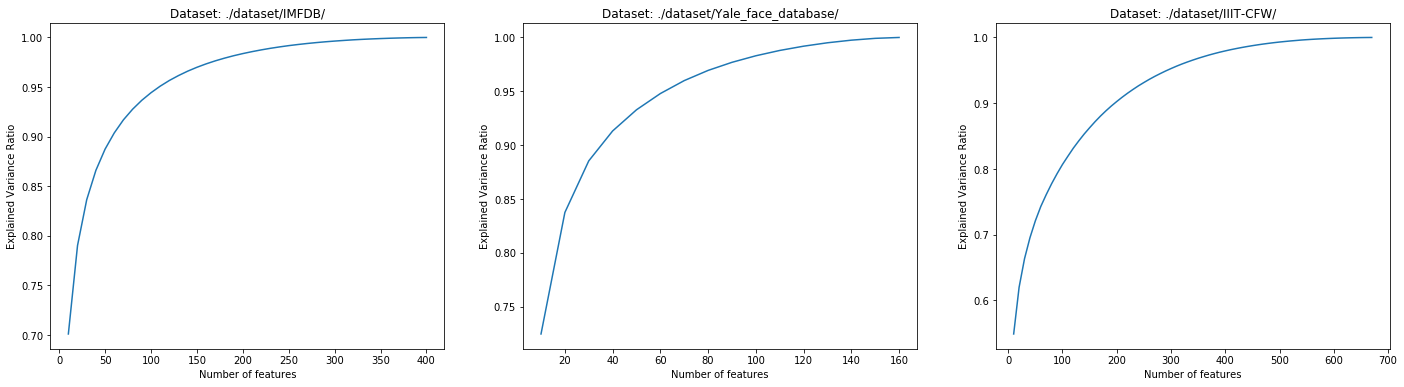
\includegraphics[scale=0.3]{./representation.png}
    
    \item \textbf{Which person/identity is difficult to represent com-pactly with fewer eigen vectors?  Why is that?  Explain with your empirical observations and intuitive answers}\\
    Within each class, the hardest to represent compactly (by small margins) have been:
    \begin{enumerate}
        \item IMDB: 2
        \item Yale: 0
        \item IIIT-CFW: 3
    \end{enumerate}

\end{enumerate}

\section{Classification}
\textbf{Use any classifier(MLP, Logistic regression, SVM, Decision Trees) and find the classification accuracy. Which method works well? Do a comparitive study.}\\
After running tests with all classifiers, and multiple dimensionality reduction tools, the best methods were evaluated.\\

\begin{table}[H]
\resizebox{\textwidth}{!}{%
\begin{tabular}{@{}lcccc@{}}
\toprule
\multicolumn{1}{c}{\textbf{Features}} & \textbf{Red. Dims} & \textbf{Classif. Error} & \textbf{Accuracy} & \textbf{F1 Score} \\ \midrule
K-LDA Sigmoid + MLP & 7 & 0.0500 & 0.9500 & 0.944892 \\ \midrule
K-LDA Polynomial + LR & 7 & 0.0500 & 0.9500 & 0.944892 \\ \midrule
K-LDA Polynomial + MLP & 7 & 0.0500 & 0.9500 & 0.944892 \\ \midrule
LDA/Fisherface + LR & 7 & 0.0500 & 0.9500 & 0.944892 \\ \midrule
K-LDA RBF + LR & 7 & 0.0500 & 0.9500 & 0.944892 \\ \bottomrule
\end{tabular}%
}
\caption{IMFDB Dataset, best results}
\label{tab:2_imfdb}
\end{table}


\begin{table}[H]
\resizebox{\textwidth}{!}{%
\begin{tabular}{@{}lcccc@{}}
\toprule
\multicolumn{1}{c}{\textbf{Features}} & \textbf{Red. Dims} & \textbf{Classif. Error} & \textbf{Accuracy} & \textbf{F1 Score} \\ \midrule
K-LDA RBF + MLP & 14 & 0.000000 & 1.000000 & 1.000000 \\ \midrule
K-LDA Polynomial + SVC & 14 & 0.000000 & 1.000000 & 1.000000 \\ \midrule
K-LDA Polynomial + MLP & 14 & 0.000000 & 1.000000 & 1.000000 \\ \midrule
K-LDA RBF + LR & 14 & 0.000000 & 1.000000 & 1.000000 \\ \midrule
K-LDA RBF + LR & 7 & 0.0500 & 0.9500 & 0.944892 \\ \bottomrule
\end{tabular}%
}
\caption{Yale Face Dataset, best results}
\label{tab:2_yale}
\end{table}



\begin{table}[H]
\resizebox{\textwidth}{!}{%
\begin{tabular}{@{}lcccc@{}}
\toprule
\multicolumn{1}{c}{\textbf{Features}} & \textbf{Red. Dims} & \textbf{Classif. Error} & \textbf{Accuracy} & \textbf{F1 Score} \\ \midrule
Resnet + LR & 2048 & 0.037037 & 0.962963 & 0.960506 \\ \midrule
K-LDA Polynomial + MLP & 7 & 0.037037 & 0.962963 & 0.959481 \\ \midrule
K-LDA Polynomial + LR & 7 & 0.037037 & 0.962963 & 0.959481 \\ \midrule
K-LDA RBF + LR & 7 & 0.037037 & 0.962963 & 0.959481 \\ \midrule
K-LDA RBF + LR & 7 & 0.0500 & 0.9500 & 0.944892 \\ \bottomrule
\end{tabular}%
}
\caption{IIIT CFW Dataset, best results}
\label{tab:2_cfw}
\end{table}

$ $\\
The confusion matrix of the best performing method is:\\
$ $\\

\end{enumerate}

\section{t-SNE}

\textbf{Similiar to 1(b) use t-SNE based visilization of faces?  Does it makesense?  Do you see similar people coming together?or something else?  Can you do visualization datasetwise and combined?}\\
Due to the parameter tuning needed, I ran a script to calculate t-SNE across datasets to get a range of results. \\
$ $\\
First, I ran just t-SNE on the data provided. As we can see, there is not much conglomeration, similar people do not come together despite multiple tests.\\
$ $\\
We can conclude that TSNE does not make much sense in this context.\\
$ $\\
However, as an experiment, I then ran t-SNE on data that was reduced by LDA to 2 dimensions. Here, around perplexity = 30/50 onwards we see conglomeration, especially in the IIIT-CFW dataset. While full separation across all data is not achieved yet, the closest we can get by eyeball estimates are at perplexity = 50 and learning rate = 50.\\
$ $\\
Instead of LDA, I then decided to try using Resnet with the same parameters, and the results are promising. I have presented this as the solution.\\
We should note that despite this presentation, the clustering comes from the preceding feature extraction, and not due to TSNE.
$ $\\
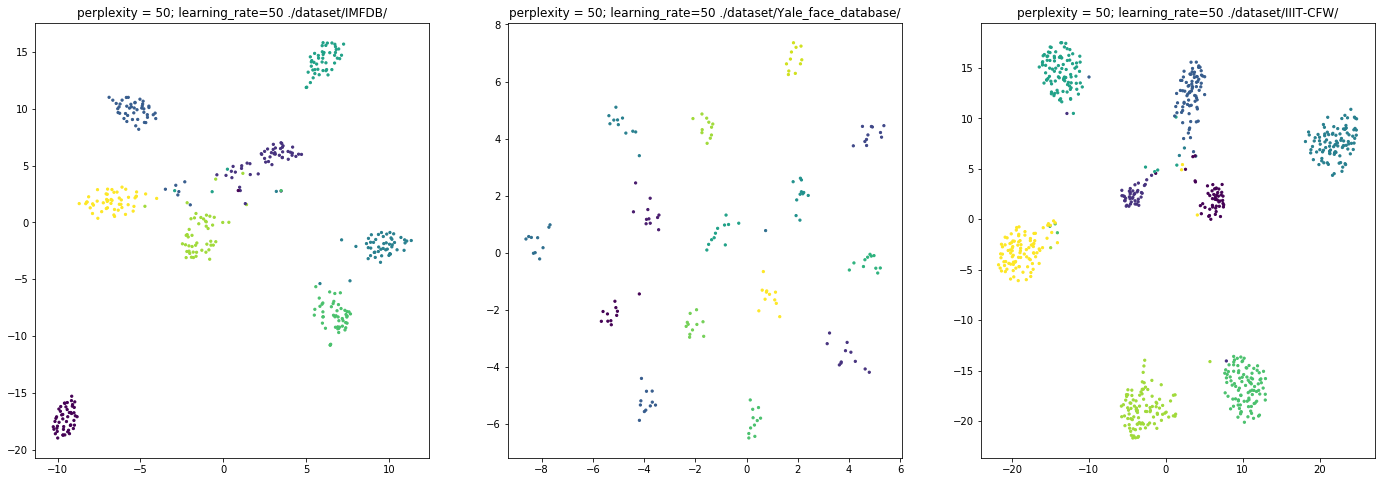
\includegraphics[scale=0.3]{./tsne.png}
\end{enumerate}


\section{face for  verification}   

\begin{enumerate}
    \item \textbf{How do we formulate the problem using KNN?}\\
    We model the problem in much the same way as in Question 2: use KNN for multiclass classification instead of binary. The key parameter here is to decide the value of k, which can be done by simple experimentation and observing performance.
    
    \item \textbf{How do we analyze the performance ? suggest  the  metrics  (like  accuracy) that is appropriate for this task.}\\
    Analyzing the performance is a matter of simply splitting the dataset into train and test, training on the train set and then testing on test. We would look at accuracy: correct classification of the test data as our primary metric, but Precision is also a metric to keep track of.
    
    \item \textbf{Show empirical results  with  all  the  representations}\\
    

\begin{table}[H]
\resizebox{\textwidth}{!}{%
\begin{tabular}{@{}lcccc@{}}
\toprule
\multicolumn{1}{c}{\textbf{Features}} & \textbf{Red. Dims} & \textbf{Classif. Error} & \textbf{Accuracy} & \textbf{F1 Score} \\ \midrule
Kernel LDA + Sigmoid + KNN k=3 & 7 & 0.0500 & 0.9500 & 0.949800 \\ \midrule
Kernel LDA + Sigmoid + KNN k=5 & 7 & 0.0375 & 0.9625 & 0.959226 \\ \midrule
Kernel LDA + Sigmoid + KNN k=7 & 7 & 0.0375 & 0.9625 & 0.959226 \\ \midrule
Kernel LDA + Sigmoid + KNN k=9 & 7 & 0.0375 & 0.9625 & 0.960027 \\ \midrule
K-LDA RBF + LR & 7 & 0.0500 & 0.9500 & 0.944892 \\ \bottomrule
\end{tabular}%
}
\caption{IMFDB Dataset, best results}
\label{tab:4_imfdb}
\end{table}


\begin{table}[H]
\resizebox{\textwidth}{!}{%
\begin{tabular}{@{}lcccc@{}}
\toprule
\multicolumn{1}{c}{\textbf{Features}} & \textbf{Red. Dims} & \textbf{Classif. Error} & \textbf{Accuracy} & \textbf{F1 Score} \\ \midrule
Kernel LDA + Sigmoid + KNN k=3 & 7 & 0.000000 & 1.000000 & 1.000000 \\ \midrule
Kernel LDA + Sigmoid + KNN k=5 & 7 & 0.030303 & 0.969697 & 0.980769 \\ \midrule
Kernel LDA + Sigmoid + KNN k=7 & 7 & 0.030303 & 0.969697 & 0.980769 \\ \midrule
Kernel LDA + Sigmoid + KNN k=9 & 7 & 0.030303 & 0.969697 & 0.980769 \\ \midrule
\end{tabular}%
}
\caption{Yale Dataset, best results}
\label{tab:4_yale}
\end{table}


\begin{table}[H]
\resizebox{\textwidth}{!}{%
\begin{tabular}{@{}lcccc@{}}
\toprule
\multicolumn{1}{c}{\textbf{Features}} & \textbf{Red. Dims} & \textbf{Classif. Error} & \textbf{Accuracy} & \textbf{F1 Score} \\ \midrule
Kernel LDA + Sigmoid + KNN k=3 & 7 & 0.029630 & 0.970370 & 0.976190 \\ \midrule
Kernel LDA + Sigmoid + KNN k=5 & 7 & 0.037037 & 0.962963 & 0.969190 \\ \midrule
Kernel LDA + Sigmoid + KNN k=7 & 7 & 0.037037 & 0.962963 & 0.970752 \\ \midrule
Kernel LDA + Sigmoid + KNN k=9 & 7 & 0.037037 & 0.962963 & 0.970752 \\ \midrule
K-LDA RBF + LR & 7 & 0.0500 & 0.9500 & 0.944892 \\ \bottomrule
\end{tabular}%
}
\caption{IIIT-CFW Dataset, best results}
\label{tab:4_cfw}
\end{table}

    $ $\\
\end{enumerate}

\section{Extension}
\subsection{The Problem}
Distinguish cartoon faces from real faces.\\

\subsection{Solution Utility}
A use case for this solution would be to automatically filter out unnecessary information, say we need to annotate human face data but scraping leads to both human and cartoon faces being downloaded. In this scenario, we use the system to filter out the cartoon data first, and then annotate accordingly.

\subsection{Experimental Pipeline}
\begin{enumerate}
    \item Creating Dataset: Take the IIIT-CFW Dataset and the IMFDB Dataset and combine the two. Create classification array accordingly based on previously available classification arrays for both datasets.

    \item Classification: Create Sigmoid Kernel LDA features. Make train test splits with 20\% test and use the MLP classifier with two hidden layers with 50 each. Train the classifier on the train sets and test on the test sets. For metrics, use classification\_report provided by sklearn to get accuracy, precision, and F1 Scores. 

    \item Qualitative results: Plot out the data reduced by PCA, TSNE, and Isomap.

        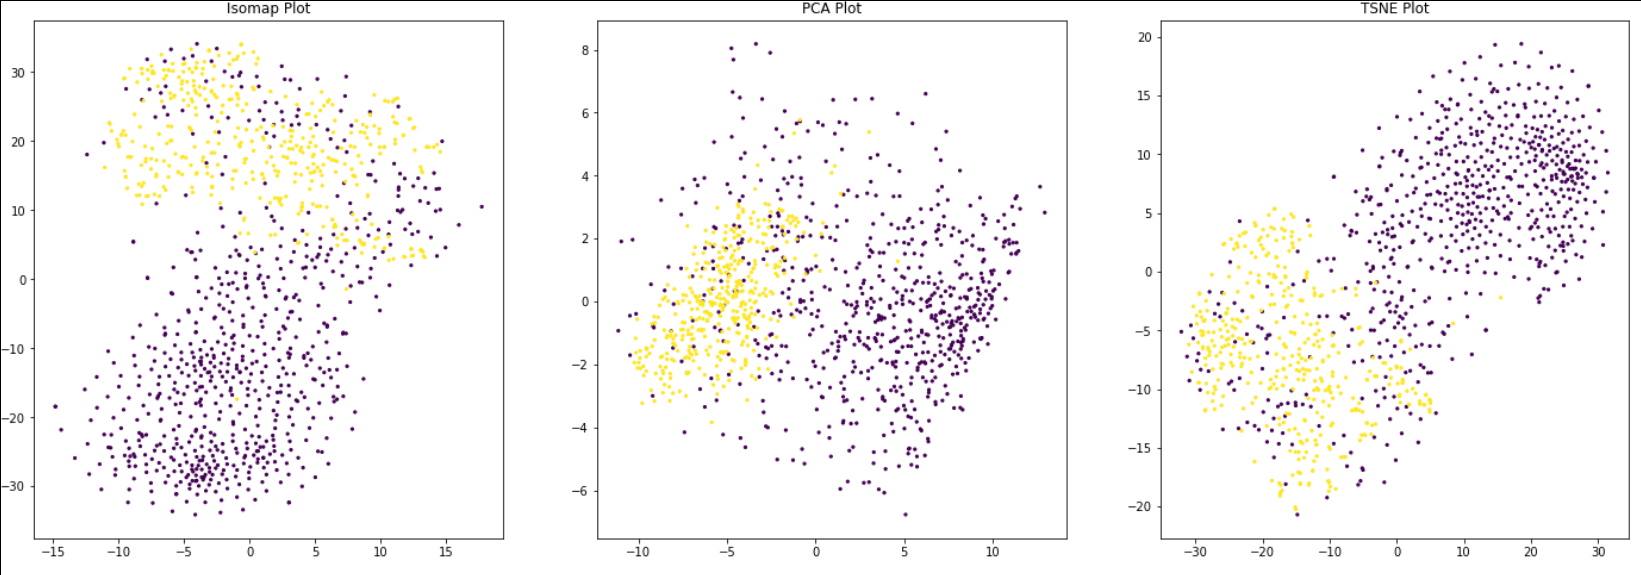
\includegraphics[scale=0.25]{./4_res.png}
\end{enumerate}


% \bibliographystyle{apalike}
% \bibliography{dbt18}

\end{document}
